%\documentclass[a4paper,11pt]{memoir} 
\documentclass[oneside, a4paper,11pt]{memoir} 

\usepackage[utf8]{inputenc}
\usepackage[danish]{babel}
\usepackage[T1]{fontenc}
\usepackage[left=4.0cm, right=2.0cm, top=3.0cm, bottom=3.0cm]{geometry} 
\usepackage{amsmath,amssymb}																						
\DeclareMathOperator{\arccosh}{arccosh}
\usepackage{listings}
%\usepackage{physics}

% SIUnitX  http://ctan.org/pkg/siunitx
\usepackage{siunitx,booktabs}		
\sisetup{per=slash}																						
\sisetup{per-mode = reciprocal}
\sisetup{inter-unit-product = \ensuremath{{}\cdot{}}}
\sisetup{output-decimal-marker = {,} }
\DeclareSIUnit{\kroner}{kr.}
\DeclareSIUnit{\LSb}{LSb}
\DeclareSIUnit{\cycles}{cycles}
\DeclareSIUnit{\div}{Div}


\usepackage{graphicx}
\newsubfloat{figure}% Allow subfloats in figure environment
\usepackage{dcolumn,booktabs}
\usepackage{url}
\usepackage{wrapfig}

% Redigere billed-/tabelteksterne.
\usepackage{caption}
\usepackage{subcaption}
\captionsetup{font=small,
labelfont={it,bf},textfont=sf,
format=hang}

% Packages for color handling
\usepackage[usenames,dvipsnames,svgnames,table]{xcolor}

\usepackage{threeparttable}

\usepackage{lscape}

\usepackage{enumitem}

% TODONotes http://ctan.org/pkg/todonotes
\usepackage{todonotes}
\usepackage{placeins}
\usepackage{lastpage}

\usepackage[hidelinks]{hyperref}  
\hypersetup{bookmarks=false}
\hypersetup{pdftitle={Embedded Modul\ae rt Audio Effekt System}} 
\hypersetup{pdfsubject={4. Semester Projekt, F18, Grp. [3]}}
\hypersetup{pdfauthor={J\"{o}rn Jacobi, Emil Schier Christiansen, Henrik Lund Hansen, Jes Rydall Larsen, Sonny Fink, Frederik Halling}}


% For includering af .pdf
\usepackage{pdfpages}

% Bibliografi
\usepackage{babelbib}
\bibliographystyle{abbrv}

% Noget forsideopsætning
\usepackage{soul} % lege lege
\sodef\an{}{0.2em}{.9em plus.6em}{1em plus.1em minus.1em}
\newcommand\stext[1]{\an{\scshape#1}}

% New commands 
\newcommand{\g}{9,82 \si{\meter\per\second\squared}}
\newcommand{\dcite}[1]{\quotedblbase{#1}\textquotedblright}
\newcommand{\husk}[2]{\todo[inline,color=green!40]{#1: #2}}
\newcommand{\jj}[1]{\todo[inline,color=green!40]{JJ: #1}}
\newcommand{\note}[1]{\todo[inline,color=yellow!40]{NOTE : #1}}
\DeclareMathOperator{\lapl}{\mathcal{L}}

% Remove paragraph indentation for document
\setlength{\parindent}{0pt}
\newcommand\hcancel[2][black]{\setbox0=\hbox{$#2$}%
	\rlap{\raisebox{.45\ht0}{\textcolor{#1}{\rule{\wd0}{1pt}}}}#2} 

% Listings package
\usepackage{listings}

%Fede overskrifter
\usepackage{kpfonts}
\usepackage{calc}
\setSingleSpace{1.0}
\SingleSpacing
\definecolor{chaptercolor}{gray}{0.8}
% helper macros
%\newcommand\numlifter[1]{\raisebox{-2cm}[0pt][0pt]{\smash{#1}}}
\newcommand\numlifter[1]{\raisebox{-.8cm}[0pt][0pt]{\smash{#1}}}
\newcommand\numindent{\kern37pt}
\newlength\chaptertitleboxheight
\makechapterstyle{hansen}{
  \renewcommand\printchaptername{\raggedleft}
  \renewcommand\printchapternum{%
    \begingroup%
    \leavevmode%
    \chapnumfont%
    \strut%
    \numlifter{\thechapter}%
    \numindent%
\endgroup%
}
  \renewcommand*{\printchapternonum}{%
    \vphantom{\begingroup%
      \leavevmode%
      \chapnumfont%
      \numlifter{\vphantom{9}}%
      \numindent%
      \endgroup}
    \afterchapternum}
  \setlength\midchapskip{0pt}
  \setlength\beforechapskip{0.5\baselineskip}
  \setlength{\afterchapskip}{1\baselineskip}
  \renewcommand\chapnumfont{%
    %\fontsize{3cm}{0cm}%
    \fontsize{2cm}{0cm}
    \bfseries%
    \sffamily%
    \color{chaptercolor}%
  }
  \renewcommand\chaptitlefont{%
    \normalfont%
    %\huge%
    \LARGE%
    \bfseries%
    \raggedleft%
  }%
  \settototalheight\chaptertitleboxheight{%
    \parbox{\textwidth}{\chaptitlefont \strut bg\\bg\strut}}
  \renewcommand\printchaptertitle[1]{%
    \parbox[t][\chaptertitleboxheight][t]{\textwidth}{%
      %\microtypesetup{protrusion=false}% add this if you use microtype
      \chaptitlefont\strut ##1\strut}%
}}
\chapterstyle{hansen}
\aliaspagestyle{chapter}{empty} % just to save some space

%linje afstand
%\DisemulatePackage{setspace}
%\usepackage[nodisplayskipstretch]{setspace}
%\setstretch{0.5}
%\siglespacing
%\onehalfspacing                                       
%\doublespacing

%compile debug, check pdflatex time
\newcommand\showtimer{Timer: \the\numexpr\the\pdfelapsedtime*1000/65536 \relax}
%\pdfresettimer}
%\usepackage{fancyhdr}
%\pagestyle{fancy}
%\fancyfoot[CE,CO]{\showtimer}

% itemize i to kolonner mulig
\usepackage{multicol}

% EPS format
\usepackage{epstopdf}

\begin{document}
% --------- Frontpage ------------------
\begin{titlingpage}
\thispagestyle{empty}
\centering
{ \setlength{\baselineskip}{24pt}
{\Huge \stext{Embedded Modul\ae rt Audio Effekt System} \par
%\textit{\&}\par
%\stext{Analogier}
}\par
\stext{Indlejrede systemer og signalbehandling - F18}
\vspace*{1cm}



\par
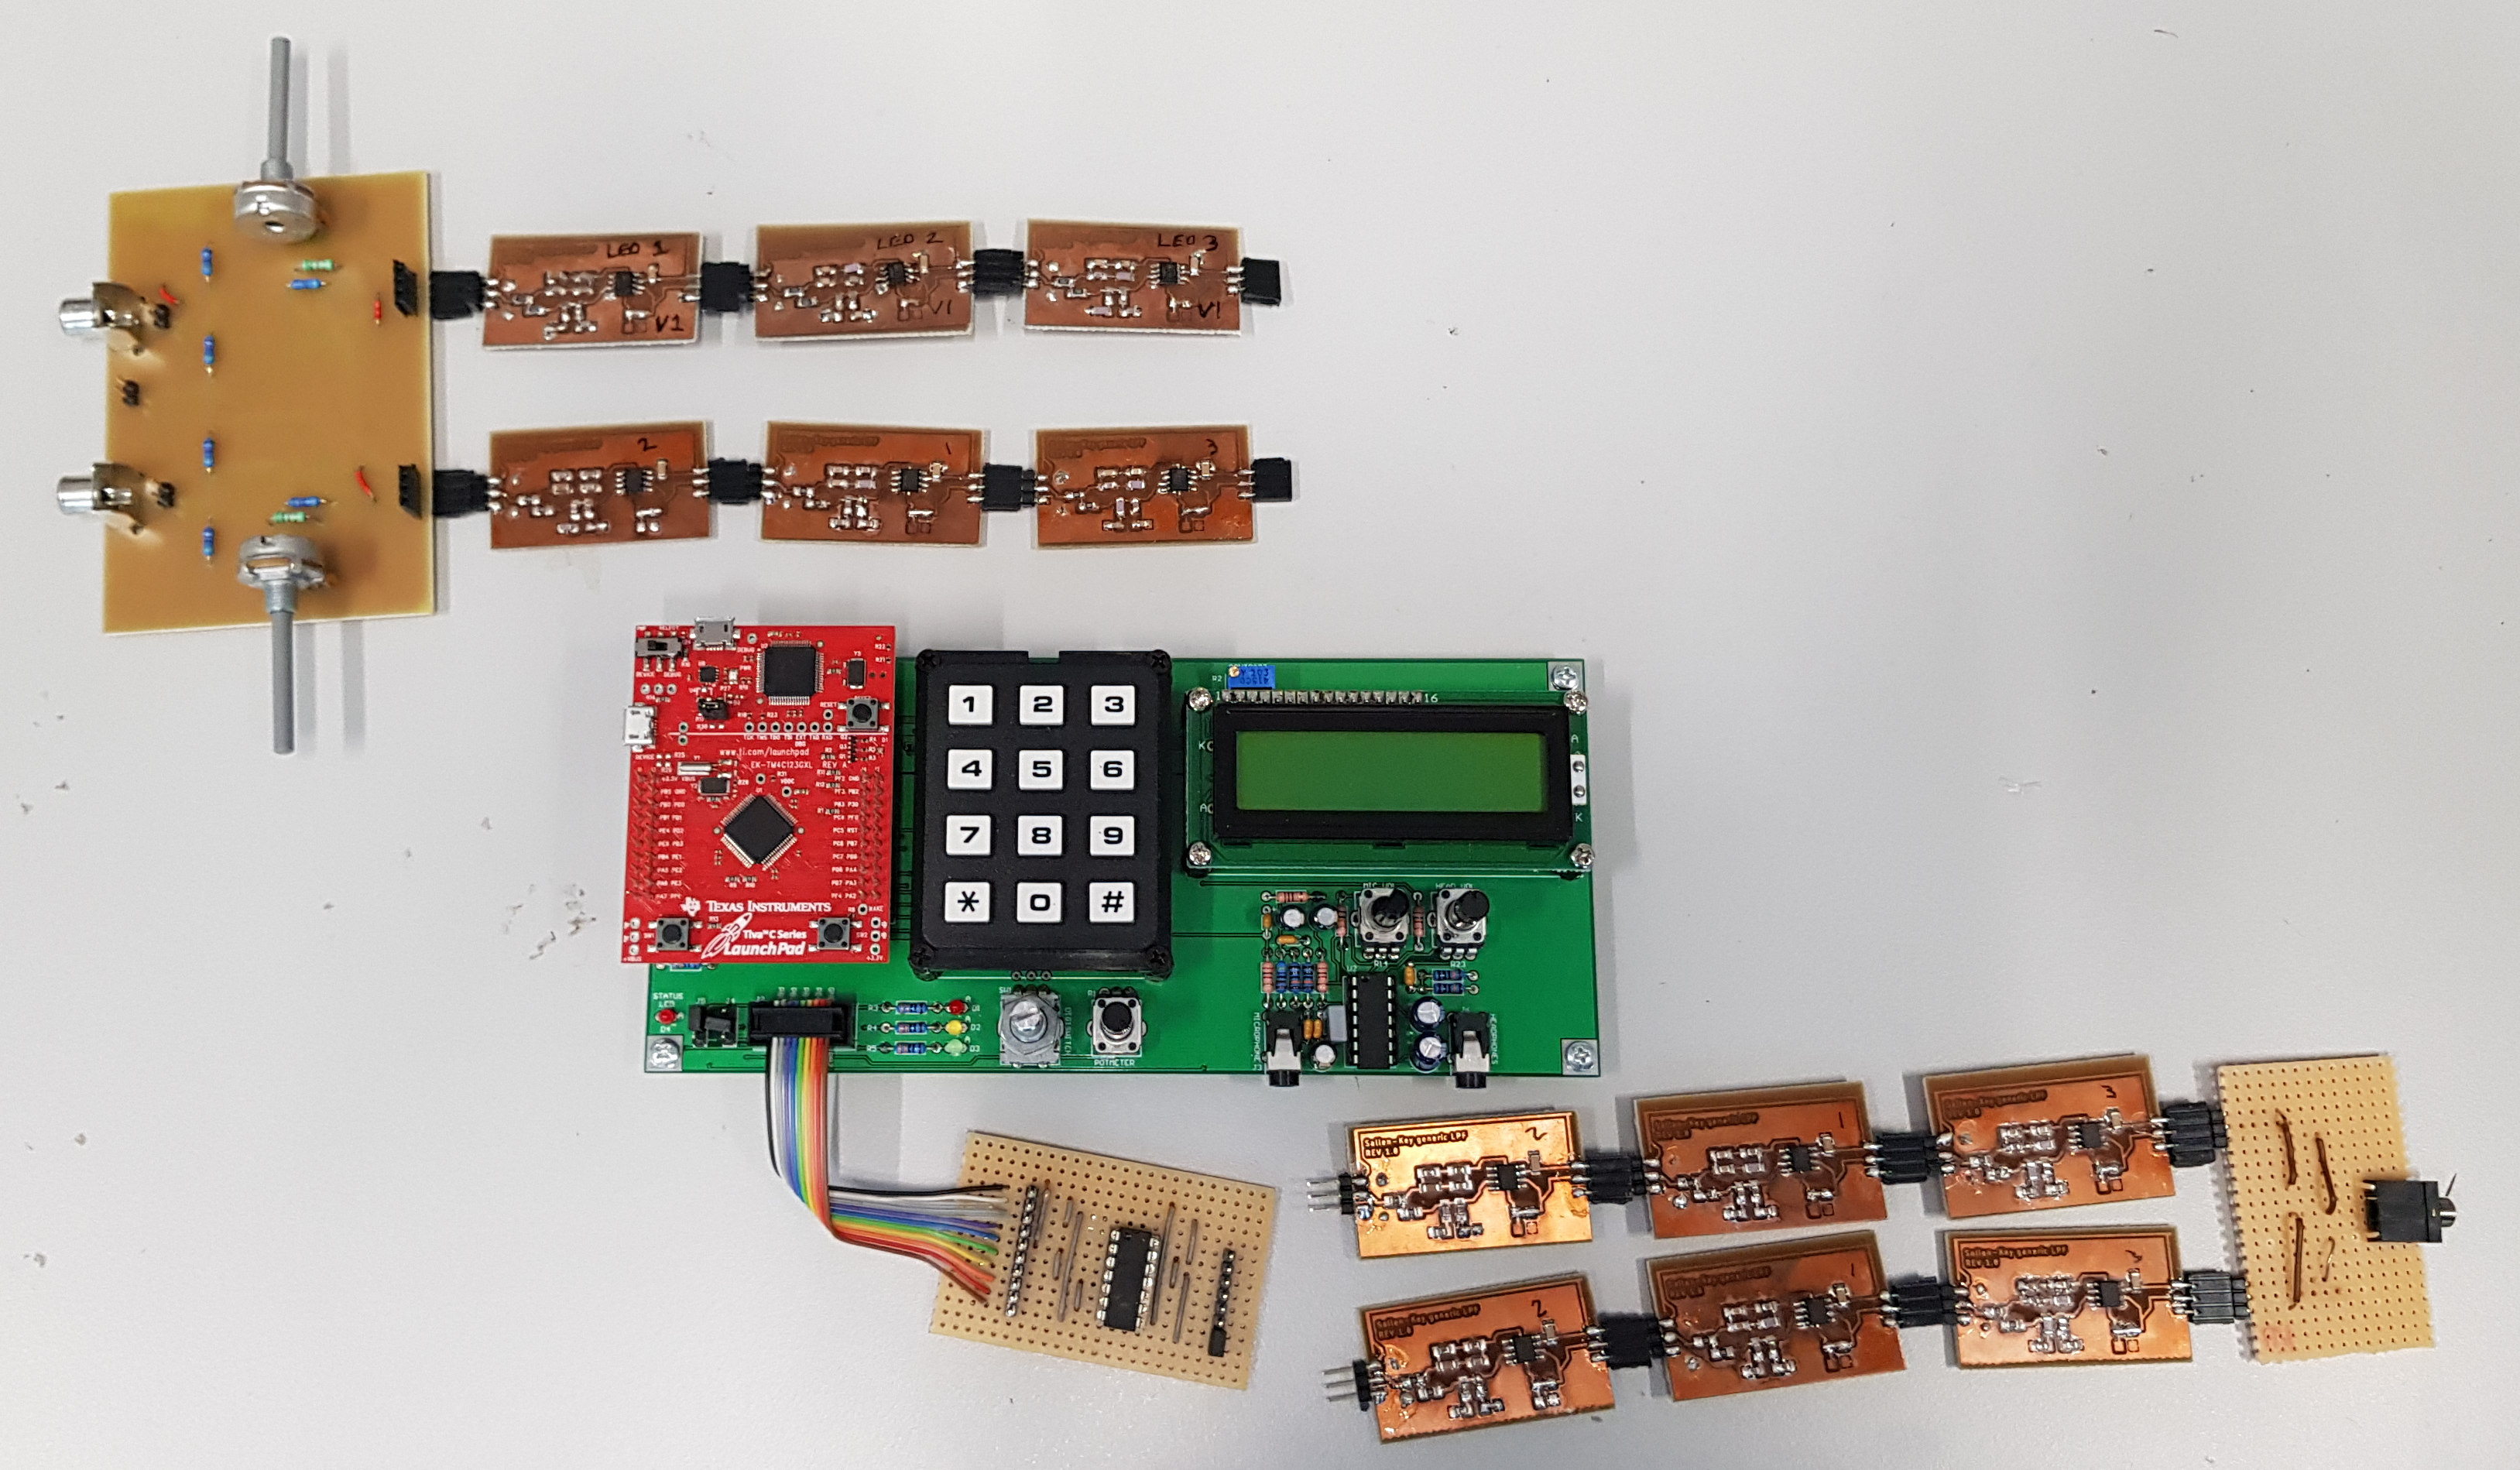
\includegraphics[width=\linewidth]{./billeder/forsidebillede.png}
\par\vspace*{2\onelineskip}
\stext{4. Semester Projekt}\par

\large\stext{J\"{o}rn Jacobi -- 230674}\par
\large\stext{Emil Schier Christiansen -- 070595}\par
\large\stext{Henrik Lund Hansen -- 270494}\par
\large\stext{Jes Rydall Larsen -- 140893}\par
\large\stext{Sonny Fink -- 040491}\par
\large\stext{Frederik Olsen Halling -- 300997}\par

\vfill
\vspace*{2\onelineskip}
\stext{Gruppe 3}\par
\stext{Vejleder: Ib Refer }\par
\stext{1. februar - 25. maj 2018}\hfill
%\stext{24. maj 2013}\hfill
\par\vspace*{2\onelineskip}
\small
\stext{M\ae rsk Mc-Kinney M\o ller Instituttet}\par
\stext{Syddansk Universitet}
\enlargethispage{2\onelineskip}
}
\end{titlingpage}


% --------- Abstract -------------------
\newpage
\thispagestyle{empty}
\renewcommand{\abstractnamefont}{\normalfont\bfseries}
\renewcommand{\abstracttextfont}{\normalfont}
\begin{abstract}
The manipulation of sound and audio signals is a big area in electronics and the analog systems of the past are now moving to the digital world. In this project, the basic implementation of digital signal processing (DSP) is explored and combined with the fundamental principles of implementing a module based audio effect system in an embedded system running on a single Cortex-M4 based microcontroller from Texas Instrument. As a supporting framework, the real time operating system FreeRTOS is used. To make the signal conversion from analog to digital and back possible, analog antialiasing and reconstruction filters are used. The chosen filter design and system at howle, is analysed and tested to provide a basis for an evaluation. To provide some functionality, an echo and a reverb effect are designed for the system.      	
\end{abstract} 

% --------- Thanks ---------------------
%\newpage\thispagestyle{empty}\null\vfill\begin{center}\emph{Thanks note goes here}\end{center}

%---------- Underskrift
%\newpage\thispagestyle{empty}\null
\section*{Underskrifter}
\vspace{3ex} \hfill Underskrevet d. 24/05-2018\\

\newlength{\streg} \setlength{\streg}{0.49\linewidth}
\vspace*{\fill} \rule{\streg}{1pt} \hfill \rule{\streg}{1pt}\\
\begin{minipage}[b]{\streg}
 \centering
 \rule{0pt}{4ex}
 J\"{o}rn Jacobi \\
 {\footnotesize (230674) (jojac11@student.sdu.dk)}
\end{minipage}
\hfill
\begin{minipage}[b]{\streg}
 \centering
 Emil Schier Christiansen \\
 {\footnotesize (ddmmyy) (xxx@student.sdu.dk)}
\end{minipage}

\vspace*{\fill} \rule{\streg}{1pt} \hfill \rule{\streg}{1pt}\\
\begin{minipage}[b]{\streg}
 \centering
 \rule{0pt}{4ex}
 Henrik Lund Hansen \\
 {\footnotesize (ddmmyy) (xxx@student.sdu.dk)}
\end{minipage}
\hfill
\begin{minipage}[b]{\streg}
 \centering
 Jes Rydall Larsen \\
 {\footnotesize (ddmmyy) (xxx@student.sdu.dk)}
\end{minipage}

\vspace*{\fill} \rule{\streg}{1pt} \hfill \rule{\streg}{1pt}\\
\begin{minipage}[b]{\streg}
	\centering
	\rule{0pt}{4ex}
	Sonny Fink \\
	{\footnotesize (040491) (sofin16@student.sdu.dk)}
\end{minipage}
\hfill
\begin{minipage}[b]{\streg}
	\centering
	Frederik Halling  \\
	{\footnotesize (300997) (frhal16@student.sdu.dk)}
\end{minipage}\newpage\thispagestyle{empty}\null\vfill

%---------- Forord
\newpage
\thispagestyle{empty}
\chapter*{Forord}\label{chap:forord}
\addcontentsline{toc}{chapter}{Forord}
Dette projekt er udarbejdet af seks ingeniør-studerende på 4. semester som studerer Elektronik og Datateknik på Syddansk Universitet. 
Projektet er udført i perioden d. 1. februar til d. 25. maj 2018. 
Projektet er udført under vejledning af Ib Refer.

\subsection{Læsevejledning}
Rapporten bør læses fra start til slut som et samlet og sammenhængende værk. 
Som udgangspunkt antages det, at læseren har et fagligt kompetenceniveau som en studerende på 4. semester med linjefag indenfor elektronik og datateknik på Syddansk Universitet.

\subsection{Typografiske konventioner}
Her er en kort oversigt over de typografiske konventioner der anvendes i denne rapport.

\bigskip

\begin{tabular}{l p{0.6\linewidth}}
	\textit{Kursiv tekst}			& Angiver filnavne i den tilhørende kodebase samt fremhævelse af ord eller fagudtryk. \\
	\textbf{Fed tekst}				& Bruges til a fremhæve produkt eller system specifikke betegnelser.\\
	\texttt{Konstant bredde tekst}	& Anvendes til kildekode eksempler. Ligeledes anvendes afgrænsende områder.\\
	\emph{Fremhævet tekst}		    & Bliver brugt når der gives en kort introduktion til hvert kapitel.\\
\end{tabular}

\subsection{Typografi}
Rapporten er fremstillet i \LaTeX - Memoir, sat i 11 pt. Computer Modern.\\
Antal sider : \pageref{LastPage}

% Removed for single page
%\newpage\thispagestyle{empty}\null\vfill

%---------- Indholdsfortegnelse  ---
\newpage
\tableofcontents*		

% Removed for single page										
%\newpage

%\DoubleSpacing	
%---------- Kalibrerings side --------
%\input{config/kalib}
%\newpage

%---------- Indledning -------------
\chapter{Indledning}
\vspace*{0.5 cm}
%\emph{intro}
I det følgende kapitel fastligges projektes formål og problemformulering der danner grundlag for rapporten.
Rapporten afspejler og dokumentere det udførte projektarbejde på 4. semester diplomingeniør i Elektronik og Datateknik på Syddansk Universitet, Teknisk fakultet / Mærsk instituttet.
Rapporten danner grundlag for eksiminationen for semester projektet hvor arbejdet er udført i perioden 1. februar til 25. maj 2018.

\husk{JJ}{Skal måske uddybes lidt og perioden flyttes til Forord.}

\section{Formål}
Semesterets hovedemne omhandler \emph{Indlejrede systemer og signalbehandling}, hvor faglighederne \emph{Analoge filtre og signaler}, \emph{Digital signalbehandling}, \emph{Embedded programmering} og \emph{Operativsystemer} er inkluderet.
Ud fra projektbeskrivelsen\footnote{ref. til  semesterprojekt beskrivelse her...} er formålet\textit{ "at skabe en applikation, der gør noget meningsfuldt, således at semesterets fire fagligheder er dækket ind"}.

\husk{JJ}{Find overgang mellem formål og problemformulering}

\section{Problemformulering}
Formålet med projektet er at undersøge hvordan lyd kan behandles og manipuleres ved at bruge digital signalbehandling i et embedded miljø.
Løsningen skal opbygges som en modulær løsning, således at nye "lydmoduler" kan efter udvikles.
Styringen af modulerne skal kunne forgå igennem EMP boardet - her tænkes det at kunne anvende HID styringen dette board stiller til rådighed og som sammen LCDen skal udgøre en platform til UI'en. 

\husk{JJ}{Husk at få indelt problemformulering i 3 grupper - Overodnet (motivation), Konkret og specifik (Udkast i listen).}


\begin{itemize}
	\item Er det muligt at lave et modulært audio effekt system der kan leve op til de fastsatte krav ? 

	\begin{itemize}
		
		\item Realtids lydbehandling 
		\item Digital filter design
		\item Analog filter design
		\item OS krav / design
		\item Test krav og eftervisning af forventede
	\end{itemize}
\end{itemize}
\husk{JJ}{Formulering af hoved- og underspørgsmål tilrettes.}

\section{Projektafgrænsning}
\begin{itemize}
	\item Produktet er ikke udviklet som et slutprodukt.
\end{itemize}

\section{Kravspecifikation} 
Kravspecikationerne for projektet er fastsat, dels ud fra kravet til selve projektbeskrivelsen og dels for at efterligne projekter udenfor det akademiske miljø.

\begin{itemize}[noitemsep]
	\item Prototypen udvikles på Tiva™ C Series TM4C123G LaunchPad Evaluation Kit \cite{spmt281a}.
	\item Tiva™ TM4C123G serie Microcontroller anvendes \cite{spmu296}.
	\item FreeRTOS anvendes som embedded kernel.
	\item Kildekoden er en del af produktet og skal overholde \textit{EMP C Code Standard}\cite{emp-c}.
	\item Der anvendes en samplingsfrekvens på $F_s = 44.1 \si{\kilo\hertz}$ stereo.
\end{itemize}


\section{Løsningsmodel}

\section{Proces- og arbejdsmetode}
							

\listoftodos
%\input{config/howto} 

%---------- Chapter ----------------
\chapter{Filterne}\label{kap:filtre}
\vspace*{0.5 cm}
\emph{I dette kapitel vil valg, design og dimensioneringen af løsningens anti-aliasning og rekonstruktions filter blive gennemgået}
\jj{Mere dækkende kapitel intro når kapitlet er blevet skrevet færdigt.}

%---------- Parts ----------------
%	\item Begrundelse baseret på antal op-amp / orden (6/8)
%	\item Kort teoretisk gennemgang af den valgte topologi
%	\item Beregninger og dimensionering af 6. ordens chebycheb filtre
%	\item Implementeringsvalg og design af hardware/schematics
%\end{itemize}


\section{Analoge filtres rolle ved digital signalbehandling}\label{sec:filter_intro}
\begin{wrapfigure}[30]{r}{3.5cm}
	\vspace{-.5cm}
	\centering
	\includegraphics[width=2.5cm]{billeder/dsp_model.png}
	\caption{DSP model.}
	\label{fig:dsp_model}
\end{wrapfigure}

For at kunne udfører digital signalbehandling af et analogt signal, bliver man nød til at overfører signalet fra den analoge verden til den digitale og tilbage igen - dette sker ved sampling og rekonstruktion.
Denne signalbehandling følger nogle faste deltrin, som kan ses i et generelt signal-blok diagram i figur \ref{fig:dsp_model}.
I dette kapitel vil fokus ligge på de analoge signaler og filtre, således vil vigtigheden de analoge filtre blive kortlagt og den efterfølgende analyse og dimensionering  \\

Når et 
\jj{hvad var jeg ved at skrive her ???}

Som udgangspunkt blev opløsningen af den Analog-Digital Converter (ADC) til at vurdere hvor meget dæmpning er analogt filter skulle have for at kunne sikre en komplet og tabsfri gengivelse af signalet.

Ud fra de fremsatte krav til projektet, benyttes der en   microcontroller fra Texas Instruments \cite{spmu296} der er udstyret med en 12bit ADC på de analoge indgange.
For at bestemme opløsning på ADC'en, kan den unipolære\footnote{Unipolær kvanteficering skyldes ADC'ens spændingsområde på $0 \longmapsto \num{3.3}\si{\volt}$.} kvanteficering $\Delta_{ADC}$ bestemmes samt Signal to Noise Ratio $SNR_Q$.
   
\begin{align}
	\Delta_{ADC} &= \frac{V_{max}}{2^N} = \frac{\num{3.3}\si{\volt}}{2^{12}} \approx \num{80.6}\si{\milli\volt}\\
	SNR_Q &= 6,02 N + 2 [\si{\decibel}] = 6,02\cdot 12+2 = 74,24 \si{\decibel} 
\end{align}
 


\note{Kort teoretisk intro til hvorfor filtre skal anvendes til sampling}
\note{Båndbrede begrænsning}
\note{Shannons sampling theorem}
\note{Generel intro til audio signaler}
\note{begrundelse for orden af filter i intro}

\section{Analyse af filter typer}\label{sec:filter_analyse}
%\note{Gennem gang af de filter topologier der har været i betragtning som en mulig løsning.}
For at kunne finde frem til et passende lavpasfilter som antialiasing filter, bliver 4 tilter typer sammenlignet - Butterworth, Chebyshev type I og II samt Bessel (Thomson).
Hver af disse filtre har en tilhørende amplitudekarakteristik der beskrives med følgende overføringsfunktion\cite{anfilter}.

\begin{align} 
H_{butterworth}(j\omega_n) &= \frac{1}{\sqrt{1 + \omega_n^{2n}}} \label{eq:H_butt} \\
H_{bessel} (j\omega_n) &= \frac{H}{a_0 + \omega^2 + ja_1\omega_n} \label{eq:H_bes}\\
H_{chebychevI}(j\omega_n) &= \frac{1}{\sqrt{1 + \epsilon^2 C_n^2(\omega_n)}} \label{eq:H_cheb1} \\
H_{chebychevII}(j\omega_n) &= \frac{1}{\sqrt{1 + \frac{1}{\epsilon^2 C_n^2(\omega_n)}}} \label{eq:H_cheb2} \\
C_n(\omega_n) &=  
\begin{matrix}
	\cos(n\arccos(\omega_n)) & 0 \le \omega_n \le 1 \\  \cosh(n \arccosh(\omega_n)) & 1 \le \omega_n 
\end{matrix} \label{eq:chev_cn_funk}
\end{align}

I ligning (\ref{eq:chev_cn_funk}) fremgår den indre funktion $C_n(\omega_n)$ som bruges i Chebychev I og II i ligening (\ref{eq:H_cheb1}) og (\ref{eq:H_cheb2}).

Figur \ref{fig:filter_typer} viser en samlet fremstilling af amplitude karakteristikken $H(j\omega_n)$ og gruppeløbstiden $D(\omega_n)$ for de fire filtertyper.

\begin{figure}[h!]
	\centering
	\includegraphics[width=1\textwidth]{matlab/filter_compare.png}
	\caption{Normeret 6.ordens filter karakteristik (øverst) og guppeløbstid (nederst) for filtertyperne Butterworth, Chebychev Type I ($0,1 \si{\decibel}$ rippel) \& Type II ($-40 \si{\decibel}$ stopbånds rippel) og Bessel.}
	\label{fig:filter_typer}
\end{figure}

Det ønskede filter skal have en rimelig flad karakteristisk i pasbåndet og en stejl overgang til stopbåndet.
Således kan lydsignalets amplitude holdes konstant i hele det ønskede frekvensområde da uønsket dæmpning/forstærkning af lydsignalet kan medfører hørbare ændringer af lydbilledet, på samme måde som en equalizer påvirker et lydsignal. 

Ligeledes ønskes en rimelig konstant gruppeløbetid. 
Gruppeløbetiden, der er defineret i ligning (\ref{eq:groupdelay_def})\cite{anfilter}, er et udtryk for hvor stor tidsforsinkelsen på signal som funktion af frekvensen er.

\begin{align}
	D(\omega) \stackrel{def}{=} - \dfrac{d(arg(N(\omega)))}{d\omega}\label{eq:groupdelay_def}
\end{align}

Hvis signal forsinkelsen bliver for stor i et givet frekvensområde, vil der fremstå en hørbar ændring af lydbilledet.
Dette fenomen er dog ret subjektivt og der findes mange meninger om hvilke tærskelværdier der kan accepteres.
Ud fra en lettere gennemgang inden for området, er antages en acceptabel relativ tidsforsinkelse på $D_{rel}(\omega) < -10 \si{\milli\second}$ til projektet.   

\subsection{Valg af filter topologi}
Hvis man som udgangspunkt kun fokusere på filtrenes gruppeløbstid, ville man skulle vælge et Bessel filter.
Bessel filteret, det er designet som et filter med maksimal fald fase, har dog langt fra den ønskede dæmpning i overgangsbåndet.
Det vælges at anvende et Chebychev type I filter, der viser sig at have den bedste dæmpning i overgangsbåndet.
Det høje udsving på gruppeløbetiden for denne filtertype, som det fremgår nederst i figur \ref{fig:filter_typer}, vil på det denomaliserede filter ligger indenfor, de i projektet, acceptable værdier. 
\\
I figur \ref{fig:filter_cheb1_denorm} ses den denormaliserede filterkarakteristik for det valgte filter med en pasbåndsrippel på $0,1 \si{\decibel}$ og en knækfrekvens på $f_c = 18 \si{\kilo\hertz}$. 

\begin{figure}[h!]
	\centering
	\includegraphics[width=1\textwidth]{matlab/filter_cheb1_denorm.png}
	\caption{Denormeret 6.ordens filter karakteristik og guppeløbstid af Chebyshev Type I ($0,1 \si{\decibel}$}
	\label{fig:filter_cheb1_denorm}
\end{figure}
\jj{ret matlab fil med denormineret grpdelay}

For at kunne bestemme dæmpningen af de demormaliserede filter, findes udtrykket for $|H(f)|$.
Med udgangspunkt i ligning \ref{eq:H_cheb1}, bestemmes $\epsilon$, som er bestemt ved ud fra rippelfaktoren i et Chebyshev filter\footnote{Figur 1.11.1 og ligning 1.11.3 i kilde \cite{anfilter}}
\begin{align}
	K_p = 20 \log \frac{1}{\sqrt{1+\epsilon^2}} \Leftrightarrow \epsilon = \sqrt{10^{K_p/10}-1}
\end{align}
Med en maksimal rippel på $K_p = 0,1 \si{\decibel}$ fås en $\epsilon$ på 
\begin{align}
	\epsilon = \sqrt{10^{0,1/10}-1} = \num{0.1526}
\end{align}

Da det ønskes at beregne $|H(f)|$ i området $f > f_c$ anvendes $C_n$ fra ligning \ref{eq:chev_cn_funk} hvor $w_n > 1$
Dæmpningen ved nyquistfrekvensen på $f_s/2 = \num{22.05}\si{\kilo\hertz}$ kan nu bestemmes som

\begin{align}
|H(f)|_{\si{\decibel}} &= 20 \log \frac{1}{\sqrt{1+ \epsilon^2  \left[\cosh(n \arccosh k )\right]^2 }} \quad, \quad k = \frac{f}{f_c} \\
|H(22,05\si{\kilo\hertz})|_{\si{\decibel}} &= 20 \log \frac{1}{\sqrt{1+ 0,1526^2  \left[\cosh(n \arccosh \frac{22,05\si{\kilo\hertz}}{18\si{\kilo\hertz}} )\right]^2 }} = \num{-12.2568} \si{\decibel}
\end{align}

\subsection{Forventet aliasing ved valgte filter type}
\jj{lidt mere intro til aliasing}
I figur \ref{fig:filter_f_fs} ses amplitude karakteristikken $|H(f)|$ af det valgte filter med blåt og den første periodiske gentagelse af frekvens spektrum $|H(f-f_s)|$ med rødt.
\begin{figure}[h!]
	\centering
	\includegraphics[width=.8\textwidth]{matlab/filter_f_fs.png}
	\caption{}
	\label{fig:filter_f_fs}
\end{figure}

En dæmpning på kun $\num{12.3} \si{\decibel}$ ved Nyquistfrekvensen er ikke ret stor og der må derfor ventes aliasing i signalet.
Størrelsen af aliasing i signalet $SA$, kan beregnes som procentvis del ved
\begin{align}
	\%SA = \frac{|H(f)|_{f=f_s-f_x}}{|H(f)|_{f=f_x}} \cdot 100 \% \label{eq:signal_alias}
\end{align} 
I ligning \ref{eq:signal_alias} angiver $f_x$ den frekvens, hvor den procentvise aliasing effekt ønskes beregnet.
Effekten kan evalueres ved at plotte $SA(f)$ fra ligning \ref{eq:signal_alias} som ses i figur \ref{fig:filter_sa}, både angivet som procentvis forhold og absolut i decibel.
Her er det således muligt at se, at der ved fx $f_c=\num{18}\si{\kilo\hertz}$ er en aliasing effekt på $5,4\%$.

\begin{figure}[h!]
	\centering
	\includegraphics[width=.8\textwidth]{matlab/filter_sa.png}
	\caption{}
	\label{fig:filter_sa}
\end{figure}

%\note{Beregninger og argumentation for SNR}

\section{Specifikation og dimensionering}\label{sec:filter_spec}



\note{sprecifikation som bi-quad systemer}
\note{hvor tæt ligger de beregnede komponent værdier i hold til de anvendte tabelværdier ?}
\note{Sallen Kay - metode 4 i afs matr.}
\note{Hvordan kommer aliasing til at have indflydelse på det endelige signal ved valg af 6. ordens filter} 


\section{Design og implementering}\label{sec:filter_design}
\note{Fremstilling i bi-quad print}
\note{Argumenteret valg er OpAmp -> den bedste der var som SMD}
\note{Kort begrundelse for enkelt R i metoden og brug af op til 4 stk. C som proto type -> hvordan ville det se ud hvis kun brugte den nærmeste C i serien og hvor stor indflydelse vil det have. Måske Sensitivitesmetoden eller H(jw) -> var det er klogt valg og måske lidt overdrevet.}

\section{Rekonstruktions filter}
\note{Hvorfor anvendes et tilsvarende AA filter på udgangen - lidt teori her}


\section{Sallen-Key aktive filtre}

Til anti aliasing filtrene anvendes aktive filtre, dette er valgt da det så ikke er
nødvendigt at skulle anvende spoler, da disse ofte fylder meget og heller ikke er
tilgængelige i et lige så bredt omfang, som kondensatorer og modstander, på SDU.
Samtidigt er det nemt at implementere da systemet i forvejen har strømforsyning til
mikroprocessoren, som kan anvendes til filtrenes operationsforstærker.

Her er det valgt at anvende Sallen-Key lav pas biquads,
da disse kan realiseres ved hjælp af flere forskellige designmetoder, præsenteret 
i læreborgen 'Analog filters, second edition'\cite{KendallSu}.
En generisk Sallen-Key lavpas biquad ser ud som i figur(\ref{fig:sklpbq}).

\begin{figure}[H]
	\centering
	\includegraphics[width=\textwidth]{billeder/sklpbq}
	\caption{Sallen-Key lowpass biquad \cite{KendallSu}}
	\label{fig:sklpbq}
\end{figure}

Det blev valgt at anvende design metode 4 fra litteraturen, minimum sensitivitet.
Denne designmetode gør filteret mindre sensitiv over for variationer i komponenter ved bl.a.
at anvende enheds forstærkning for derfor at undvære $R_a$ og $R_b$.
Det vælges at $R_1 = R_2$, herefter findes $C_1$ og $C_2$ ved hjælp af ligning \ref{eq:dm4c1} og \ref{eq:dm4c2}.

\vspace{15pt}

\begin{minipage}{0.5\linewidth}
	\begin{equation}
	\label{eq:dm4c1}
		C_1 = \frac{2Q}{\omega_0}
	\end{equation}
\end{minipage}
\begin{minipage}{0.5\linewidth}
	\begin{equation}
	\label{eq:dm4c2}
	C_2 = \frac{1}{2Q\omega_0}
	\end{equation}
\end{minipage}

\vspace{15pt}

Det kan så ses at denne designmetode dog kommer på bekostningen af en stor spredning i
kondensator værdierne, som stiger afhængigt af filterets Q-værdi, som ses i ligning
\ref{eq:kondspred}.

\begin{equation}
\label{eq:kondspred}
	\frac{C_1}{C_2} = 4Q^2
\end{equation}




\section{Input stage med pre-amp og DC-offset}
\label{sec:inputstage}
Systemet skal kunne modtage et signal fra en lydkilde, som afspiller lyd i det menneskeligt hørbare område. 
Før signalet kan videreføres til anti aliasing filtrene, skal der være en mulighed for eventuelt at forstærke signalet med en operationsforstærker. 
På den måde kan en fuld opløsning opnås ved den senere AD konvertering. 
\newline
Et almindeligt analogt lydsignal har generelt frekvenser mellem 20Hz og 20kHz, som svarer til det menneskeligt hørbare område. 
Signalets spænding varierer for forskellige kilder. 
Der findes ingen officiel standard, men en del forbruger-elektronik har typisk en maksimal amplitude på 0,447V.\cite{wikiLine} 
\newline
Til forstærkningen benyttes en aktiv operationsforstærker med 3,3V single-supply. 
Men indgangssignalet fra lydkilden vil svinge omkring 0V. 
Derfor skal signalet have et offset, da signalet ellers vil blive klippet hver gang det går under 0V, da operationsforstærkeren ved single-supply ikke har mulighed for at have negative udgangssignaler. 
Det ønskes at indgangssignalet har mulighed for at svinge både så højt og lavt som muligt, så offsettet designes til at være symmetrisk, med respekt til  forsyningsspændingen. 
\begin{equation}
	{V_{offset}} = \frac{V_{supply}}{2} = \frac{3,3\text{V}}{2} = 1,65\text{V}
\end{equation}
Ved et offset på 1,65V kan signalet ideelt have en maksimal amplitude på 1,65V. 
%Herfra skal den valgte operationsforstærkers output swing i forhold til dens forsyningsspænding trækkes fra. (vender tilbage til det her når op-amp skal vælges)
Ved at opbygge en spændingsdeler, kan offsettet skabes. Kredsløbet ses på figur \ref{fig:modtagerKreds}.

\subsubsection{Valg af operationsforstærker til forstærkning af indgangssignalet}
Operationsforstærkeren som skal forstærke signalet vælges ud fra en række krav. 

\begin{itemize}
	\item Forstærkeren skal kunne forsynes med  single-supply 3,3V
	\item Båndbredden skal være minimum 44,1 kHz.
	\item Rail to rail voltage swing skal være så stort som muligt. 
	\item Slew rate skal være hurtig nok til at signalet ikke forvrænges. 
	\item Komponenten skal være tilgængelig som SMD komponent. 
\end{itemize}
Den nødvendige slew rate kan beregnes ved formel \ref{eq:slewrate}.\cite{slewrate}
\begin{equation}
\label{eq:slewrate}
\text{Slew rate} = 2 \pi \cdot f_{maks} \cdot V_{maks} = 2\pi \cdot 22,05\si\kilo\hertz \cdot 1,65\si\volt = 0,46\si[per-mode=symbol]{\volt\per\micro\second}
\end{equation}
\husk{JES}{Er det egentligt kun 20kHz her?}
Ud fra kravene vælges operationsforstærkeren AD8031 som SMD komponent. 
Forstærkeren kan operere ved en single-supply forsyning ned til 2,7V, har 80MHz -3dB båndbredde ved en forstærkning på 1 og en slew rate på 30\si[per-mode=symbol]{\volt\per\micro\second}
Forstærkerens output swing ligger inden for 20mV af rail-spændingen. Ved 3,3V ligger spændingsvidden således fra 0,02V til 3,28V. 
Forstærkerens specifikationer overgår kravene med en stor margen. 
Det var ikke muligt at finde en anden operationsforstærker som var tilgængelig som SMD, der både havde en acceptabel slew rate, samt muligheden for en single-supply forsyningsspænding på 3,3V. 
Havde der været mere tid, kunne det have været bestilt hjem. 

\subsubsection{Beregning af forstærkning}
For at forstærke signalet, opsættes operationsforstærkeren som en ikke-inverterende forstærker. 
Da indgangssignalets maksimale amplitude vil variere alt efter input, skal forstærkningens styrke kunne justeres. 
Derfor sættes en variabel modstand i serie med feedback-modstanden. 
Det ses på figur \ref{fig:modtagerKreds}. 
Den variable modstand kan gå fra at være tæt på kortsluttet og op til 100k$\Omega$.
For at undgå en kortslutning fra operationsforstærkerens output og til den inverterende indgang, er den variable modstand sat i serie med en feedback-modstand på 5k$\Omega$. 
$R_2$ er valgt til 47k$\Omega$, så modstanden matcher modstanden fra højpasfilteret. 
I formel \ref{eq:Aminfors} og \ref{eq:Aminfors} ses den mulige maksimum- og minimumsforstærkning.

\begin{equation}
\label{eq:Aminfors}
A_{maks.} = 1 + \frac{R_{feedback} + R_{variabel}}{R_2} = 1 + \frac{5\text{k} \Omega + 100\text{k} \Omega}{47\text{k} \Omega} = 3,23
\end{equation}
\begin{equation}
\label{Amaksfors}
A_{min.} = 1 + \frac{R_{feedback}}{R_2} = 1 + \frac{5\text{k} \Omega}{47\text{k} \Omega} = 1,11
\end{equation}

\subsubsection{Højpas filter-design}
Mellem inputtet og operationsforstærkeren sidder en kapacitor, som blokerer for al DC fra indgangssignalet. 
Som det ses på figur \ref{fig:modtagerKreds}, vil kapacitoren og modstandene fra offsettet udgøre et højpas filter. 
Filterets knækfrekvens sættes så lavt, at alle frekvenser i det hørbare område ikke påvirkes. 
Ved AC-analyse kortsluttet forsyningen. Derfor sidder modstandene $R1$ og $R2$ parallelt.
Det endelige kredsløb er kopieret, således der er to udgange for at opnå stereo. 
\begin{equation}
f_c = \frac{1}{2\pi R C} = \frac{1}{2 \pi \frac{1}{\frac{1}{47k \Omega}+\frac{1}{47k \Omega}}  470\text{nF}} = 14,1\text{Hz}
\end{equation}

\begin{figure}[h]
\caption{Kredsløbet for modtageren af indgangssignalet.}
\includegraphics[width=0.8\linewidth]{./billeder/Modtager.png}
\label{fig:modtagerKreds}
\end{figure}

\husk{Jes}{Hvis der er problemer med antal sider, kan der henvises til et bilag med det samlede print i stedet. Opdatering: Bilag med samlet print er ved at blive lavet. }

\section{Output stage}

Da de rekonstruerede signal stadigvæk er offset skal DC-værdien fjernes igen inden signalet føres ud af systemet.
Dette gøres ved at anvende en kondensator inden udgangen, dette danner et højpas led med belastningen på udgagen med en knækfrekvens der kan beregnes med ligning \ref{eq:fchp1}.

\begin{equation}
	f_c = \frac{1}{2\pi RC}
\label{eq:fchp1}
\end{equation}

Ved lidt søgning kan der findes frem til at indgangs impedansen på lyd forstærkere og lignende typisk ligger på $10\si{\kilo\ohm}$ og opefter.

Knækfrekvensen skal gerne være på maksimum $20\si{\hertz}$.

Herefter kan ligning \ref{eq:fchp1} omskrives til ligning \ref{eq:fchp2}, for at finde kondensator værdien.

\begin{equation}
	C = \frac{1}{2\pi Rf_c} = \frac{1}{2\pi 10\si{\kilo\ohm} 20\si{\hertz}} = 0,796\si{\micro\farad}
\label{eq:fchp2}
\end{equation}

Det findes så at kondensatoren skal være ca. 0,8\si\micro\farad.
For nemhedens skyld valgtes en værdi på 1\si\micro\farad, da det er en let tilgængeligt standard værdi.
Med denne kondensator vil belastningen kunne være ned til cirka 8\si\kilo\ohm, før at knækfrekvensen vil overstige 20\si\hertz, Hvilket overholder kravspecifikationen for denne.

\section{Opsummering}





\chapter{Mikrocontrolleren}\label{kap:mcu}
\vspace*{0.5 cm}
\emph{I dette kapitel ....}
\section{FreeRTOS}
\note{Kort intro til hvad FreeRTOS er og hvilken funktionalitet det stiller tilrådighed}


\section{Preemptive schedulering}
FreeRTOS er bygget på en prioritetsbaseret preemptive scheduleringsalgoritme.\newline
Når et operativ system opererer med en preemptive scheduleringsalgoritme kan kørende processer preemptes - blive stoppet - og skiftet ud med en anden proces.\newline
Det kan f.eks. være at en proces der har ventet på en I/O device får tilgang til denne.
Scheduleren vil så skifte den nuværende kørende proces ud og skifte den hidtil ventende proces ind så den kan køres.
Dette gør scheduleren via et context switch.\newline
Når et context switch sker gemmes ''konteksten`` af den nuværende task i en process control block (PCB), og ydermere sker der et state restore, hvor informationen i PCBen af den task, der skal skiftes til hentes.
Det som bliver gemt i PCBen er værdierne i CPU registrene (Program counter, etc.) og anden vigtig operativ systemsinformation.\newline
Prioritetsbaseret skeduleringsalgoritmer tildeler alle tasks en prioritet som er baseret på taskens vigtighed.\newline
FreeRTOS er et real-time operativ system og et primært formål ved real-time operativ systemer er at give et respons på begivenheder indenfor en vis deadline.
FreeRTOS skeduleringsalgoritme sørger så for at den task med højest prioritet bliver givet processortid.

\section{Interrupt håndtering}

\note{Interrupt execution diagram og opsætning} 

\section{Sampling af lydsignal igennem ADC}


\section{Håndtering af brugergrænseflade og human input interface}

\section{Modulær opbygning af effekter}

\section{Genskabelse af signal via DAC igennem SPI}



\chapter{Effektmoduler}\label{chap:DSP}

\husk{Emil}{ved ikk eom den skulle have et bedre navn}

\section{Reverb effektmodul}\label{sec:reverb}
\husk{Emil}{jeg er ikke helt sikker på opbygningen af denne sektion..}
Reverb, rumklang, er resultatet af lydbølger som bliver reflekteret tilbage af samtlige overflader med forskellige vinkler.\newline
Rumklang er resultatet af lydbølger som bliver reflekteret af samtlige overflader i et rum, derved bygges der en masse reflektioner op hvis amplitude falder mod $0$ som de bliver absorberet af overfladerne i rummet.\newline
Der er to primære metoder for implementeringen af en digital reverb effekt.
Der er convolution (foldnings) reverben og den algoritmiske reverb.
\subsection{Convolution reverb}
Reverberation, rumklang, er en tidsinvariant effekt, hvilket betyder at det ikke har nogen betydning, hvornår en tone bliver spillet, det vil ultimativt resultere i præcis den samme reverberation. \newline
Med tidsinvariante systemer kan de karakteriseres ved deres impulsrespons.
Convolution reverbs virker ved at lave en foldning af rummets impulsrespons og det lydsignal der sættes på indgange n til reverben.\newline
Dette skaber en realistisk rumklangseffekt, fordi impulsen i dette tilfælde vil være en lyd som holder samme energiniveau ved alle frekvenser.
Efter impulsen bliver spillet vil den blive reflekteret rundt i rummet.
Nogle af reflektionerne møder mikrofonen med det samme mens andre bliver ført rundt i rummet og amplituden af signalerne går mod $0$ pga. overfladerne af objekterne i rummet absorbere energien fra dem.\newline
Multiplikering af hver punkt af impulsresponset med amplituden af samplet giver så rummets respons til den sample.
Dette gøres for hver sample af inputtet og giver overlappende responser som så adderes og resulterer i rumklang.
En ulempe ved convolution reverbs er, at der skal mange beregninger til for at få resultatet.
Hvert sample skal individuelt multipliceres med hvert sample af impulsresponset og adderes.
Hvis der haves $N$ samples og impulsresponset er $M$ samples lang skal der udføres $N+M$ multiplikationer og additioner.
F.eks. hvis der haves et impulsrespons på 1 sekund og der samples med $44.1\si{kHz}$, skal der udføres næsten 2 milliarder multiplikationer og additioner i sekundet.
Antallet af multiplikationer og additioner kan dog reduceres drastisk ved at arbejde i frekvensdomænet i stedet for, da foldning i frekvensdomænet er multiplikation.

Fordelen ved convolution reverbs er at ethvert rum i verden kan imiteres, hvis impulsresponset for det valgte rum haves.\newline
Derudover kan man opfinde rum ved at syntetisere et impulsrespons.

\subsection{Algoritmisk reverb}
En algoritmisk reverb virker ved at bruge flere forskellige delays og feedback loops til at opbygge en serie af ekkoer, som dør ud over tid.
Det er sammensætningen af de basale byggeblokke som giver karakteristikken på rummet der emuleres.\newline
Et eksempel på en simpel algoritmist reverb effekt er all-pass filteret.
%insert billede af all-pass filter
Her bliver samplet feeded forward til outputtet så lyden bliver spillet med det samme.
Derudover smides samplet ind i en delay buffer.
Rumklangen skabes så af samples fra delay bufferen, som fungerer som opbygningen af ekkoer og feedback loopet som agerer som absorptionen for at skabe aftagende ekkoer.




\husk{Emil}{koden skulle ikke være her alligevel}
\section{Implementering af reverb}
\section{Ekko effektmodul}
	\subsection{Implementering af ekko effekt}
	
\section{Lowpass filter modul}
Som et effektmodul blev der udviklet et FIR (finite impulse response) filter, hvilket vil sige at impulsresponset af filteret falder til nul efter et vist stykke tid.\newline
Et FIR filters overføringsfunktion er givet ved
\begin{equation}
H(z) = b_0 + b_1z^{-1} + \cdots + b_Kz^{-K}
\end{equation}
Hvori $b_i$ er filterets koefficienter.\cite[p.218]{Tan2013}\newline
Filteret og dets koefficienter bliver ved run-time beregnet efter brugeren inputter cutoff frekvensen. Filteret designes og det koefficienter bliver beregnet via frequency sampling metoden.
\pagebreak
\section{Frequency Sampling}
Frequency sampling metoden virker ved at man lader $h(n)$ for $n = 0, 1, \cdots, N - 1$ approksimere filterets impulsrespons, hvilet for FIR filtre er deres koefficienter, og $H(k)$ for $k = 0, 1, \cdots, N - 1$ er de diskrete Fourier transformationskoefficienter.
\begin{figure}[!ht]
	\includegraphics[width=\textwidth]{billeder/frequencysampling.png}
	\caption{Frekvenssampling af amplitudekarakteristik}
	\label{fig:frequencysampling}
\end{figure}
H(k) findes ved at sample den ønskede amplitudekarakteristik i frekvensdomænet ved lige adskilte frekvenser som vist i figur \ref{fig:frequencysampling}.
FIR koefficienterne findes så ved
\begin{equation} \label{eq:fir_koefficienter}
b_n = h(n) = \frac{1}{2M + 1} \left\{H_0 + 2\displaystyle\sum_{k = 1}^{M}\, H_k\cos\left(\frac{2\pi k (n - M)}{2M + 1} \right) \right\} \quad \mathrm{for} \quad n = 0, 1, \cdots, M
\end{equation}
Resten af koefficienterne findes ved $h(n) = h(2M - n) \quad \mathrm{for} n = M + 1, \cdots, 2M$ ved brug af symmetri, når filteret antages at have lineær fase.


\subsection{Implementering af FIR filter}
Det digitale filter blev valgt at blive implementeret som et FIR filter, fordi FIR filtre giver mulighed for at have lineær negativ fase hvilket medfører konstant gruppeløbetid.\newline
Negativ lineær fase medfører konstant gruppeløbetid da gruppeløbetid er givet ved
\[
\tau = \frac{\mathrm{d}\varphi}{\mathrm{d}\omega}
\]
Konstant gruppeløbetid er en fordel at have i audio applikationer da en varierende gruppeløbetid kan komme til at lyde forkert.\newline
Modulet virker ved at det tager en cutoff frekvens som brugerinput og dernæst beregner normerede cutoff frekvens ved
\[ \Omega_c = 2\pi\frac{f_c}{f_s} \]
Hvor $f_c$ er cutoff frekvensen og $f_s$ er samplingsfrekvensen.
Dernæst beregnes en array af amplitudekarakteristikken $H_k$ for de normerede frekvenser fra $0$ til $\pi$ ved 
\[ \Omega_k = \frac{2\pi k}{(2M + 1)} \quad \mathrm{for} \quad k = 0, 1, \cdots, M \]
Når $H_k$ haves beregnes $M$ filterkoefficienter via. \ref{eq:fir_koefficienter} og resten findes ved symmetri.\newline
Filteret virker ved at en buffer fyldes med $x$ samples og dernæst bliver der foretaget en foldning for hver sampel i bufferen med hver filterkoefficient.





%---------- Chapter ----------------
\chapter{Diskussion og vurdering}\label{kap:diskussion}
\vspace*{.5cm}

Mange af de valg der er blevet taget ved design af de analoge filtre er en blanding af kompromiser. Der findes desværre ikke en endelig korrekt løsningsmodel og således har valgene været ret subjektive.
Ideelt ville et Bessel filter have givet den bedste gruppeløbetid, men det er samtidigt den design metode der har mest ringe dæmpning.

Valget af modulet bi-quad filter PCB, var praktisk som prototype, men medførte også en del støj pga det store areal og de mange forbindelsesledninger.

Problemerne under dimensionering af filtrene medførte, at de teoretisk frembragte værdier ikke kunne anvendes direkte. Det var ikke nogen hindring at eftervise og sammenholde den teoretiske del med den praktiske ved at anvende tabelværdier i stedet.
\\
\\
%MCU
For at kunne håndtere en korrekt sampling af signalet med præcis timing der bl.a. fjerner jitter fejl i lydgengivelse, blev det valgt at sampling ISR'en lå uden for FreeRTOS' task-håndtering. 
Dette medførte at det kun var den resterende tid (imellem hver sample) hvor FreeRTOS havde mulighed for at udføre de underliggende tasks.
Implementeringen af de mellemliggende ISR'er til håndtering af digiswitch og keypad var underlagt en lavere prioritet for at kunne sende data igennem køer styret af FreeRTOS. Det kunne således give andledning til starvation. 
Det var derfor vigtigt at få fastlagt en passende taskdelay og taskprioritering.    
\\
Det er ikke alle dele af den udviklede kode til projektet der er blevet helt færdiggjort inden afleveringsfristen.
Den overordnede funktionalitet er på plads, selv om visse funktionsvalg, som fx aktivering og deaktivering af moduler, kan kræve en ændring i kildekoden.
På samme måde er en 100\% løs kobling imellem moduler og kerne software heller ikke blevet opnået, men ville være mulig med mere udvikling - grundideerne er på plads. 
\\
\\
Den algoritmiske implementering af de digitale effekter medførte, at en anden tilgang til buffer princippet var nødvendig.
Kaskadekobling af denne type effekter var ikke mulig med én enkelt buffer, og begrænset hukommelse i projektets mikrocontroller betød, at flere buffere med tilstrækkelig længde ikke var en mulighed.

En betydeligt mere realistisk rumklangs/ekko effekt kunne have været opnået med et ''convolution reverb``, dette ville dog have krævet en bedre mikrocontroller med højere clockfrekvens og mere plads til at gemme data og der blev derfor i stedet valgt at anvende algoritmiske løsninger.

Den valgte FIR filter design metode viste sig at fungere med de ressourcer der er til rådighed. 
En af ulemperne ved \textit{frequency samplings} metoden, er ripple dannelse imellem de samplede frekvenser.



	
						
%---------- Chapter ----------------
\chapter{Konklusion} \label{kap:konklusion}

							


\SingleSpacing

\nocite{*}
\bibliography{rapport}\label{bilag:litteratur}
%\listoffigures
%\listoftables

%--------- Bilag -------------------
\appendix
%\chapter{Bilag}
\chapter{Test af det samlede system}
\label{bilag:test}
Testens formål er at udføre en vector network analyse af det samlede system for at finde systemets amplitude-karakteristik. 
Det samlede system består af modtageren af indgangssignalet, anti-aliasing filtrene for den ene kanal, Tiva-kittet med EMP board og microcontroller, DAC, rekonstruktionsfilteret for den ene kanal og udgangskredsløbet. 

\subsection{Udstyr}
\begin{itemize}
	\item Bode 100 med tilhørende udstyr
	\item Èn computer med Bode Analyzer Suite installeret
	\item To oscilloskop-prober
	\item Skillekondensator
\end{itemize}

\subsection{Fremgangsmåde og forsøgsopstilling}
Opsæt Bode 100 uden noget tilsluttet. 
Åben Bode Analyzer Suite, og vælg en Gain/Phase-analyse under Vector Network Analysis. 
Analysen sættes op med følgende indstillinger:
\begin{multicols}{2}
\begin{itemize}
	\item Startfrekvens: 10 Hz
	\item Slutfrekvens: 50 kHz
	\item Minimum 401 data points
	\item Source level: 0 dBm
	\item Attenuator på receiver 1 \& 2: 10 dB
	\item Receiver bandwidth: 100 Hz
	\item External reference på CH1 \& CH2
\end{itemize}
\end{multicols}
Vælg Trace 1 til Magnitude (dB). \newline
Med Bode Analyzer suite laves en kalibrering af Bode 100, når udgangen og indgangene på Bode 100 er koblet sammen. 
Skillekondensatoren skal være på udgangen. \newline
Opsæt det samlede system som vist på figur \ref{fig:lol}. 
Bode 100's udgang med skillekondensator og CH1 kobles til indgangen på den ene kanal af det samlede system. 
CH2 kobles til udgangen af det samlede system for den tilsvarende kanal. 
Analysen kan nu udføres. 

\subsection{Resultat af test}
Datasættet for resultatet af testen kan ses i den vedhæftede fil \textit{'habibi.csv'}. 
\husk{Jes}{Filnavn skal rettes her!}
\begin{figure}[h]
	\caption{Overføringsfunktionen af det samlede system.}
	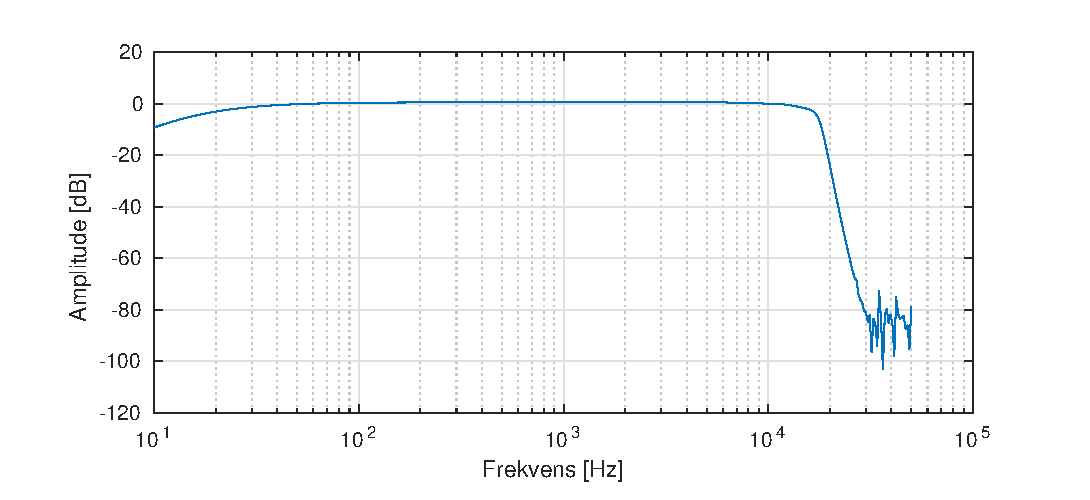
\includegraphics[width=1\linewidth]{./billeder/tf_samletsystem.eps}
	\label{fig:tf_samletsystem}
\end{figure}

\section{Test af anti-aliasing filtre}
%Formål her.
Testen følger samme fremgangsmåde, som ved testen af det samlede system. 
Dog testes udelukkende anti-aliasing filtrene.  
\chapter{Ordliste} \label{bilag:ordliste}

\begin{table}[h!]
	\caption{Ordliste}
	\label{tab:ordliste}
	\begin{threeparttable}
		\begin{tabular}{l p{0.7\textwidth}}
			\toprule
			\textbf{Ord}      & \textbf{Beskrivelse}   \\ 
			\midrule
			AA			& Antialiasing.\\
			ADC			& Analog digital converter (Eng.)\\
			ANSI		& American National Standards Institute (Eng.)\\
			API			& Grænseflade på en computer der tillader én softwarekomponent at kommunikere med en anden\tnote{a}\\
%			CLI			& Commandline interface (Eng.)\\
			DAC			& Digital analog converter (Eng.)\\
%			Latency		& (Eng.) Tidsforsinkelsen imellem stimulans og respons.\\ 
			LCD			& Liquid crystal display (Eng.) \\
			MCU       	& Micro Controller Unit (Eng.). Microcontroller eller mikroprocessor. \\
%			Periferienhed & Selvkørende hardwaremodul i mikrocontrollerens arkitektur.\\
			Preemptive	& (Eng.) Afbrydelse af task fra fx. en scheduler.\\
			PWM			& Pulse Width Modulation (Eng.) \\
			SAR			& Successive Approximation Register (Eng.)\\
%			Shell		& Brugerinterface (CLI) til operativsystemets funktionalitet.\\
			SPI			& Serial Peripheral Interface (Eng.)  \\
			UART		& Universal asynchronous receiver and transmitter (Eng.)\\
			\bottomrule
		\end{tabular}
	
		\begin{tablenotes}
			\item[a] \textit{Den Danske Ordbog - \url{http://ordnet.dk/}}
		\end{tablenotes}
	\end{threeparttable}
\end{table}

\chapter{Test af reverb og ekko impulsrespons}\label{sec:test_af_effekt}
Da ekko og reverb begge er tidsinvariante effekter, betyder det at de kan karakteriseres af deres impulsrespons.\newline
Testens formål er at finde impulsresponset for ekko- og reverbeffekten.
%Systemet består af modtager af indgangssignal, anti-aliasing filtre, TIVA-kit med EMP board, DAC, rekonstruktionsfilter og udgangskredsløbet.
Systemet består af et signalindgangs board, en række anti-aliasing- og inputfiltre, et TIVA-kit med EMP board, et board med en DAC, rekonstruktionsfiltre og et udgangskredsløbet.
\section{Forsøgsopstilling og fremgangsmetode}
\begin{itemize}
	\item Funktionsgenerator indstillet til pulse med en peak-to-peak spænding på $500\si{mV}$ og et DC-offset på $250\si{mV}$, og pulsen sættes til at være $25\si{\mu s}$ lang svarende til et sample
	\item Oscilloskop sat til single sweep med en trigger sat til $200\si{mV}$
	\item Load modstand koblet på udgangen på $10\si{k\Omega}$
	\item Reverb delay sat til $10\si{ms}$ og input- og feedbackgain sat til $-0.50$
	\item Ekko delay sat til $44\si{ms}$ samples og gain sat til $0.5$
\end{itemize}
%Funktionsgeneratoren kobles på signalindgangen af systemet, og oscilloskopets prober placeres hhv. på indgangen til mikrocontrolleren og på udgangen af rekonstruktionsfilteret.\newline
Funktionsgeneratoren kobles på signalindgangen sammen med en af oscilloskopets prober, og den anden placeres på udgangskredsløbet.\newline
Effektmodulerne aktiveres hver for sig og der tages et single sweep.
\subsection{Resultat}
Inputtet er den første impuls angivet som den gule graf og outputtet er vist ved den røde graf:
\begin{figure}[!ht]
		\centering
	\begin{minipage}{0.50\textwidth}
		\centering
		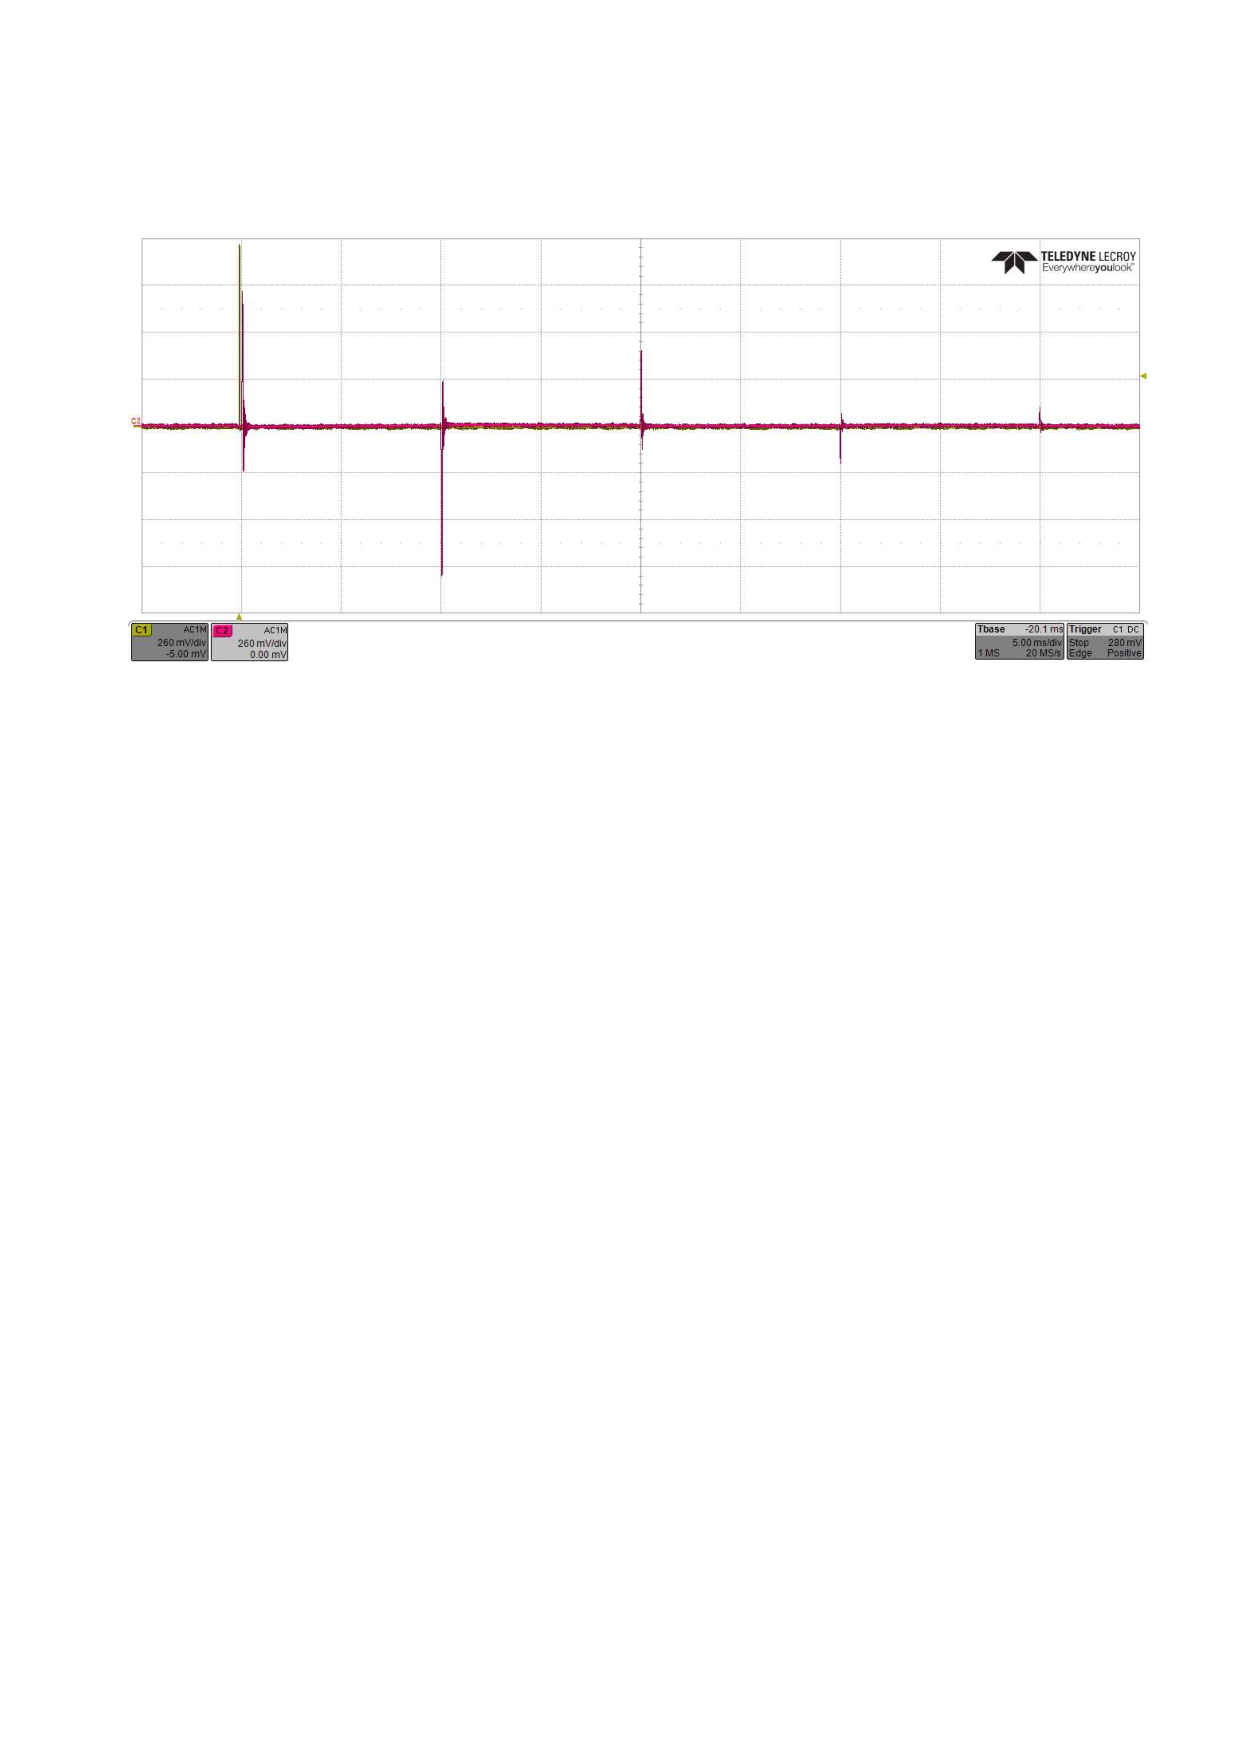
\includegraphics[width=0.9\textwidth, height=5cm]{billeder/reverb.png}
		\caption{Impulsrespons for reverbtesten.}
		\label{fig:imp_reverb}
	\end{minipage}\hfill
	\begin{minipage}{0.50\textwidth}
		\centering
		\includegraphics[width=0.9\textwidth, height=5 cm]{billeder/ekko.png}
		\caption{Impulsrespons for ekkoeffekten.}
		\label{fig:imp_echo}
	\end{minipage}
\end{figure}
På figurene kan det aflæses at delay tiderne stemmer meget præcist overens med de fra programmets side forventede delay tider. På figuren for ekko (\ref{fig:imp_echo}) ses også at gentagelsen af impulsen er faldet til ca $400\si{mV}$ hvor det oprindelige output er lige under $800\si{mV}$, hvilket stemmer nogenlunde overens med det forventede gain på $0.5$.\newline 
På reverb figuren (\ref{fig:imp_reverb}) ses det at den første gentagelse af impulsen er af samme størrelse som det oprindelige output. Dette skyldes at feedforward har en gain på $0.5$ og feedback har samme gain så de tilsammen udgør en fuld kopi af det oprindelige signal. 
Under normal brug vil disse gains være betydeligt lavere, hvilket vil give en noget hurtigere aftagende respons, men for at få et tydeligere test resultat blev disse ret høje gain værdier valgt.
%\husk{Sonny}{kan godt huske noget om at vi også testede på indgange til µControlleren, men var der ikke den samme støj på den almindelige indgang og vi ser den næsten heller ikke i matlab plottende}
%Støjen på indgangen skyldes de tre anti-aliasing filtre, som var forbundet via \husk{hvad kalder man de ting} hvilket giver en dårlig forbindelse.\newline
%
%\husk{Sonny}{Først målte tal så hvad de tilsvare præcis i "samples" og så kan der siges at det passer til det delay vi forventede}
%Her \ref{fig:impulsresponsreverb} ses impulsresponset af reverbeffekten.
%Som det fremgår af figuren bliver samplen gengivet med en dæmpning hver $2000$. sample.
%Gains samt delay var sat højt for at overdrive og tydeliggøre feedbacket.\newline
%Som det ses på figuren bliver impulsen feedbacket èn gang som svarende til et ekko efter $2000$ svarende til $45,35\si{mS}$.


%\input{section/symbol}
%\chapter{Pin mapping} \label{bilag:pinmap}
\jj{Gennemgå kilder og noter i dette kap.}
\begin{table}[h!]
	\caption{Pin konfiguration af Tiva LaunchPad, EMP print og Projekt print}
	\label{tab:pin_mapping}
	\begin{threeparttable}
		\begin{tabular}{l l l l l l}
			\toprule
			\textbf{Tiva Pin\tnote{a}} 	& 
			\textbf{GPIO\tnote{b}}  	&
			\textbf{Tiva\tnote{c}} 		& 
			\textbf{EMP\tnote{d}}  		&
			\textbf{Projekt\tnote{e}} 	\\ 
			\midrule
			1.01 &      & 3V3  	& +3.3VDC		& 3V3			 		\\
			1.02 &  PB5 &      	& PB5			&  		\\
			1.03 &	PB0 &	   	& PB0			&								\\
			1.04 &	PB1 &      	& PB1			&								\\
			1.05 &	PE4 &	   	& Audio Out     &							\\
			1.06 &	PE5 &	   	& Audio In		&								\\
			1.07 &	PB4 &	   	& PB4			& 		\\
			1.08 &	PA5 &	   	& DIGI A		& 					\\
			1.09 &	PA6 &	   	& DIGI B    	& 								\\
			1.10 &	PA7 &	   	& DIGI P2		& 								\\
			\midrule
			2.01 &     	& GND  	& GND  			&  GND 						\\
			2.02 & PB2 	&      	& PB2			&								\\
			2.03 & PE0 	&	  	& KEYB G 		&								\\
			2.04 & PF0 	& SW2	& 				&								\\
			2.05 &     	& RESET	& 				&								\\
			2.06 & PB7	&		& PB7			& 					\\
			2.07 & PB6	&		& PB6			& 					\\
			2.08 & PA4 	&      	& KEYB F 		&						\\
			2.09 & PA3 	&		& KEYB E    	& 						\\
			2.10 & PA2  &		& KEYB D		& 						\\
			\midrule
			3.01 &		& 5V0	& +5VDC			&								\\
			3.02 &		& GND	& GND			&								\\
			3.03 & PD0	&(R10)	&				&								\\
			3.04 & PD1	&(R9)	&				&								\\
			3.05 & PD2	&		& LCD RS		& 				\\
			3.06 & PD3	&		& LCD E			& 						\\
			3.07 & PE1	&		& KEYB H		& 							\\
			3.08 & PE2	&		& KEYB J		&							\\
			3.09 & PE3	&		& KEYB K		&								\\
			3.10 & PF1	&LED (R)& LED R			&								\\
			\bottomrule
		\end{tabular}
	
		\begin{tablenotes}
			\item[] Forsættes på næste side...
		\end{tablenotes}
	\end{threeparttable}
\end{table}
\newpage
\begin{table}[ht]
	\caption{Pin konfiguration af Tiva LaunchPad, EMP print og Projekt print}
	\begin{threeparttable}
		\begin{tabular}{l l l l l l}
			\toprule
			\textbf{Tiva Pin\tnote{a}} 	& 
			\textbf{GPIO\tnote{b}}  	&
			\textbf{Tiva\tnote{c}} 		& 
			\textbf{EMP\tnote{d}}  		&
			\textbf{Projekt\tnote{e}} 	\\ 
			\midrule
			4.01 & PF2	&LED (B)& LED Y			&								\\
			4.02 & PF3	&LED (G)& LED G			&								\\
			4.03 & PB3	&		& PB3			&	DAC $\overline{LDAC}$							\\
			4.04 & PC4	&		& LCD D4		& 			\\
			4.05 & PC5	&		& LCD D5		& 				\\
			4.06 & PC6	&		& LCD D6		& 				\\
			4.07 & PC7	&		& LCD D7		& 				\\
			4.08 & PD6	&		& Status LED	& 		\\
			4.09 & PD7	&		& 				&								\\
			4.10 & PF4	& SW1	& 				&								\\
			\bottomrule
		\end{tabular}
		
		\begin{tablenotes}
			\item[x] Jumper på EMP printet skal sættes til. \textbf{J5 pin 1-2} og \textbf{J4 pin 2-3}.
			\item[a,b] JP1-4 på Tiva LaunchPad \cite[Afsnit 2.1.5 s. 9]{spmu296}.
			\item[c] On-board fnuktion  \cite[Afsnit 2.1.5 s. 9]{spmu296}.
			\item[d] EMP print funktionalitet er beskrevet i tilhørende diagram \cite{emp-diagram}.
			\item[e] Projekt , se bilag \ref{bilag:diagram}.
		\end{tablenotes}
	\end{threeparttable}
\end{table}
%\chapter{Stykliste} \label{bilag:styklister}
\begin{table}[h!]
\small
%\centering
\caption{Stykliste for diagrammerne \ref{bilag:diagrammer}}
\label{tab:styklister}
\begin{threeparttable}
\begin{tabular}{p{0.25\linewidth}p{0.1\linewidth}p{0.15\linewidth}p{0.05\linewidth}p{0.1\linewidth}p{0.1\linewidth}p{0.05\linewidth}}
%\begin{tabular}{ l l l l l l l }
\toprule
\multicolumn{1}{l}{\textbf{Komponent}}       &
\multicolumn{1}{l}{\textbf{Værdi}}       &
\multicolumn{1}{l}{\textbf{Type}}       &
\multicolumn{1}{l}{\textbf{Tol.}} &
\multicolumn{1}{l}{\textbf{Klasse}} &
\multicolumn{1}{l}{\textbf{Bemærkning}} &
\multicolumn{1}{l}{\textbf{Type / Lev.}}  \\ 
\hline
R3, R6 & $\SI{10}{\ohm}$ & Metalfilm & $\pm 5\%$ & $\SI{0.25}{\watt}$ & 100ppm/\si{\celsius} & (a) \\
R30 & $\SI{330}{\ohm}$ & Metalfilm	& $\pm 5\%$ & $\SI{0.25}{\watt}$ & 100ppm/\si{\celsius}  & (a) \\
R1, R5 & $\SI{4.7}{\kilo\ohm}$ & Metalfilm	& $\pm 5\%$ & $\SI{0.25}{\watt}$ & 100ppm/\si{\celsius} & (a) \\
R15, R17, R26, R28 & $\SI{6}{\kilo\ohm}$ & Metalfilm & $\pm 5\%$ & $\SI{0.25}{\watt}$ & 100ppm/\si{\celsius} & (a) \\
R9, R10, R20, R21 & $\SI{10}{\kilo\ohm}$ & Metalfilm & $\pm 5\%$ & $\SI{0.25}{\watt}$ & 100ppm/\si{\celsius} & (a) \\
R31 & $\SI{30}{\kilo\ohm}$ & Trim & $\pm 5\%$ & $\SI{0.25}{\watt}$ & 100ppm/\si{\celsius} & (b) \\
R11, R12, R13, R14, R22, R23, R24, R25 & $\SI{32}{\kilo\ohm}$ & Metalfilm & $\pm 5\%$ & $\SI{0.25}{\watt}$ & 100ppm/\si{\celsius} & (a) \\
R2, R4, R7, R8 & $\SI{100}{\kilo\ohm}$ & Metalfilm & $\pm 5\%$ & $\SI{0.25}{\watt}$ & 100ppm/\si{\celsius} & (a) \\
R16, R18, R27, R29 & $\SI{150}{\kilo\ohm}$ & Metalfilm	& $\pm 5\%$ & $\SI{0.25}{\watt}$ & 100ppm/\si{\celsius} & (a) \\
\midrule
C24, C27 & $\SI{90}{\pico\farad}$ & Keramisk & $\pm 5\%$ & 100 \si{\volt} &  & (c)\\
C11, C14, C16, C18 & $\SI{93}{\pico\farad}$ & Keramisk & $\pm 5\%$ & 100 \si{\volt} &  & (c)\\
C29, C31 & $\SI{95}{\pico\farad}$ & Keramisk & $\pm 5\%$ & 100 \si{\volt} &  & (c)\\
C8, C9, C10, C13, C15, C17,C21, C22, C23, C26, C28, C30 & $\SI{940}{\pico\farad}$ & Keramisk & $\pm 5\%$ & 100 \si{\volt} &  & (c)\\
C2, C4, C6, C12, C20, C25 & $\SI{100}{\nano\farad}$ & Keramisk & $\pm 5\%$ & 100 \si{\volt} &  & (c)\\
C3, C7  & $\SI{318}{\nano\farad}$ & Keramisk & $\pm 5\%$ & 100 \si{\volt} &  & (c)\\
C1, C5 & $\SI{10}{\micro\farad}$ & Elektrolyt & $\pm 5\%$ & 25 \si{\volt} &  & (c)\\
C32, C33 & $\SI{1.1}{\micro\farad}$ & Polyester & $\pm 5\%$ & 100 \si{\volt} &  & (c)\\

C40 & $\SI{0.1}{\micro\farad}$ & Keramisk & $\pm 5\%$ & 50 \si{\volt} &  & (c)\\
C41 & $\SI{10}{\micro\farad}$ & Tantal & $\pm 5\%$ & 100 \si{\volt} &  & (c)\\
\midrule
IC1, IC2, IC4, IC5 & MCP6274-E\_P & OP Amp &  &  &  & (u) \\
IC6 & MCP4922-E\_P & D/A converter &  &  &  & (u) \\
P7, P8, P9, P10, P11, P12, P13, P14 & Pinheader & Stik &  &  & 1 pin & (u) \\
P15, P16, P17, P18 & Pinheader & Stik &  &  & 2 pins & (u) \\
P1, P2, P3, P4, P5, P6 & Pinheader & Stik &  &  & 10 pins & (u) \\
P19 & Pinheader & Stik &  &  & 4 headers & (u) \\
S2, S3, S4, S5, S8, S9 & Socket & Stik &  &  & 10 huller & (u) \\
S1 & Socket & Stik &  &  & 16 huller & (u) \\
S6, S7 & Socket & Stik &  &  & 2x10 huller & (u) \\
PHONO1, PHONO2 & MX-387GL & Phono &  &  &  & (u) \\
LED1 & $\SI{3.3}{\volt}$ & Grøn lysdiode &  & $\SI{0.1}{\watt}$ & $\SI{3}{\milli\meter}$ & (u) \\
\hline
\bottomrule
\end{tabular}
\begin{tablenotes}
%\textbf{Typ/Lev.}
\item[a] (MRS25), (Phillips)
\item[b] (), (Bourns)
\item[c] (), (Phillips)
\item[u] Ukendt
\end{tablenotes}
\end{threeparttable}
\end{table} 

%\input{section/tidsplan}
%\input{section/diagrammer}
%\chapter{Diagram} \label{bilag:diagram} % Denne side skal ikke bruges, den skal blot fjernes og erstattes med digrammet


\end{document}
